\documentclass[a4paper,11pt]{article}

% Identificação
\newcommand{\pbtitulo}{R}
\newcommand{\pbversao}{1.2}

\usepackage{../sty/tutorial}

%----------------------------------------------------------------------
% Início do Documento
%----------------------------------------------------------------------
\begin{document}
	
\maketitle % mostrar o título
\thispagestyle{fancy} % habilitar o cabeçalho/rodapé das páginas

%--------------------------------------------------------------------------
% RESUMO DO ARTIGO
%--------------------------------------------------------------------------
\begin{abstract}
  % O primeiro caractere deve vir com \initial{}
  \initial{R}\textbf{ é uma linguagem bem como um ambiente de desenvolvimento integrado para cálculos estatísticos e gráficos disponibilizada de forma Open Source. Foi criada originalmente por Ross Ihaka e por Robert Gentleman no departamento de Estatística da universidade de Auckland, Nova Zelândia, e desenvolvida em um esforço colaborativo de pessoas em vários locais do mundo. O código fonte é escrito principalmente em C, Fortran e R. As capacidades da R são estendidas através de pacotes criados pela sua comunidade ativa, um famoso repositório pode ser encontrado na CRAN\cite{cranoficial} (Comprehensive R Archive Network) com uma vasta gama de aplicações, abrangendo as áreas de finanças, genética, aprendizagem de máquinas, medicina, ciências sociais e estatísticas espaciais. A linguagem está se tornando padrão porque os processos de mineração de dados vivem uma era dourada, quer estejam em uso para determinar preços de publicidade, descobrir novos medicamentos ou fazer a sintonia fina de modelos financeiros.}
\end{abstract}
\vspace{20pt}

%-----------------------------------------------------------------------------
% CONTEÚDO DO ARTIGO
%-----------------------------------------------------------------------------
\section{Parte inicial}
A R apareceu inicialmente em 1996, e surgiu de uma necessidade de seus criadores, Robert Gentleman e Ross Ihaka quando estavam iniciando suas carreiras como professores na universidade de Auckland. Na universidade, existia um laboratório de estatística com vários computadores, mas grande parte dos softwares disponíveis na época eram pagos. Para a maioria dos alunos que eles ensinavam, após esses saírem da universidade, dificilmente teriam acesso as licenças desses softwares pois não possuíam condições financeiras. Isso se mostrava ainda pior com os alunos estrangeiros, já que muitos países sequer tinham representantes comerciais para vender tais softwares.

Nessa época, tiveram acesso ao livro ``New S language'' (A nova linguagem S) de \textbf{Rick Becker} e \textbf{John Chambers}. Então tomaram como base essas ideias que também era uma linguagem de computador voltada para cálculos estatísticos e produziram uma própria como forma dar suas aulas de estatísticas sem problemas. Assim surgiu o R, uma brincadeira com a linguagem S (assim como o GNU PSPP - referência ao SPSS). R é tão similar a S que muitos dos códigos escritos rodam inalterados. O código fonte de R está disponível sob a licença GNU/GPL e as versões binárias pré-compiladas são fornecidas para Windows, Macintosh, e muitos sistemas operacionais Unix/Linux.
\begin{figure}[H]
	\centering
	
\includegraphics[width=0.2\textwidth]{imagens/logo.png}
	\caption{Logo do R}
\end{figure}

R disponibiliza uma ampla variedade de técnicas estatísticas e gráficas, incluindo modelação linear e não linear, testes estatísticos clássicos, análise de séries temporais (time-series analysis), classificação, agrupamento entre muitas outras. É considerada uma linguagem facilmente extensível por causa do grande número de funções e extensões disponibilizadas pela comunidade, que também é reconhecida por seus vários pacotes.

Muitas das funções padrão de R são escritas no próprio R, o que torna fácil aos usuários seguir escolhas algorítmicas feitas. Para tarefas computacionais intensivas, códigos C, C++, Java e Fortran também podem ser ligados e chamados durante a execução. Usuários experientes podem escrever código C ou Java para manipular diretamente objetos R.

Como muitas outras linguagens, R suporta matrizes aritméticas. Sua estrutura de dados inclui escalares, vetores, matrizes, quadros de dados (similares a tabelas numa base de dados relacional) e listas. Seu sistema de objetos é extensível e inclui, entre outros, modelos de regressão, séries temporais e coordenadas geoespaciais.

Resumidamente, R é uma linguagem de programação, usada para manipulação de dados e gráficos. Amplamente utilizada por estatísticos e cientistas de dados para o desenvolvimento de software estatístico e análise de dados. O que torna a R tão útil e como explicar sua rápida aceitação? É que estatísticos, engenheiros e cientistas podem melhorar o código de software básico ou escrever variações para tarefas específicas. Pacotes escritos para a linguagem R acrescentam algoritmos avançados, técnicas de mineração para vasculhar bancos de dados e gráficos coloridos e texturizados. 

\subsection{Principais características}
As principais características dessa linguagem, são:
\begin{itemize}[noitemsep]
  \item Livre e de fonte aberta (Open Source). 
  \item Fornece acesso completo aos algoritmos e sua implementação. 
  \item Fórum que permite aos pesquisadores explorar e expandir os métodos utilizados para analisar dados.
  \item É o produto de trabalho de muitos especialistas nas áreas de estatística e análise de dados.
  \item Permite que Cientistas de todo o mundo possam ter acesso as ferramentas de software necessárias para realizar pesquisas.
  \item Promove uma investigação reproduzível (código criados como funções, podem ser reproduzidos) e fornece ferramentas abertas e acessíveis.
  \item As funções são escritas em R, e permite verificar facilmente o que as funções realmente fazem.
\end{itemize}

Como principais \textbf{vantagens}, podemos citar:
\begin{itemize}[noitemsep]
  \item Rápida e gratuita com vários pacotes a disposição.
  \item Pesquisadores de estatística fornecem os seus métodos em pacotes de R.
  \item Oferece de análise estatística, para as mais variadas áreas do conhecimento, como economia, biologia, genética e ciências sociais.
  \item Comunidade de usuários ativos.
  \item Excelente para a simulação, programação e análises intensivas.
  \item Interfaces com software de armazenamento de banco de dados (SQL).
\end{itemize}

Como principais \textbf{desvantagens}, podemos citar:
\begin{itemize}[noitemsep]
  \item Não existe um suporte comercial oficial, conta entretanto com o apoio da comunidade.
  \item Grandes conjuntos de dados são limitados pela memória RAM.
  \item Fácil cometer erros por não conhecer bem a linguagem.
\end{itemize}

\subsection{Por que aprender R?}
R está se tornando a linguagem padrão para a \textbf{Ciência de Dados}. Isso não quer dizer que é a única linguagem ou a melhor ferramenta para todo tipo de trabalho. É, no entanto, a mais amplamente utilizada e está aumentando em popularidade.

A O’Reilly Media realizou uma pesquisa em 2014 para compreender quais são as ferramentas que os cientistas de dados estão usando atualmente. Descobriram que R é a linguagem de programação mais popular. Vários outros rankings de programação assinalam um crescente aumento da linguagem.

Se é daqueles que gosta de visualizar o comportamento dos dados das mais variadas formas, e ainda sim, apresentar os resultados de forma impressionante, R é para você. Novos pacotes surgem a cada dia, como ``ggplot2'', que permite gráficos mais elaborados e profissionais. Além disso, pode-se facilmente exportar esses gráficos para anexar a um documento ou apresentação, sem perder a qualidade da imagem.

Aprender uma linguagem de programação é semelhante a estudar um novo idioma, o ideal é dedicar um grande período em sua utilização. E a melhor forma de se familiarizar com seus comandos, um passo a passo bem simples é: ler um texto introdutório (como esta apostila) e ao mesmo tempo digitar os comandos no RStudio, observar os resultados compreendendo como se comporta. R possui uma plataforma inigualável para a programação de novos métodos estatísticos, de uma forma simples e fácil, sendo naturalmente extensível. 

\section{RStudio no Docker}
RStudio é o editor principal do R, é compatível com diversos sistemas operacionais e pode ser facilmente instalado sem exigir muito conhecimento para isso. Nesta apostila, usaremos a instalação via \textbf{Docker} sendo a forma mais prática para termos total controle do ambiente, principalmente se está começando agora e precisa realizar várias reinstalações.

\begin{theo}[]{}
Por meu sistema operacional ser o Ubuntu os comandos descritos nesta seção serão para este, realize as devidas adaptações para seu sistema (conforme as descrições dos comandos).
\end{theo}

Criar uma pasta que serve como associação ao contêiner: \\
{\ttfamily\$ mkdir \$HOME/rstudio}

Fornecer permissões a esta pasta de modo que o contêiner possa acessá-la: \\
{\ttfamily\$ chown 1000 \$HOME/rstudio}

Baixar a imagem disponível: \\
{\ttfamily\$ docker pull rocker/rstudio}

Instalar e rodar a imagem: \\
{\ttfamily\$ docker run --name meu-rstudio -d -p 8787:8787 -v \$HOME/rstudio:/home/rstudio -e \\ PASSWORD=rstudio rocker/rstudio}

Para executar abrir um navegador e acessar a URL \url{http://localhost:8787}. O usuário e a senha são: \textbf{rstudio}.

Para encerrar o RStudio: \\
{\ttfamily\$ docker stop meu-rstudio} 

Para iniciar novamente o RStudio: \\
{\ttfamily\$ docker start meu-rstudio} 

\section{Ambiente RStudio}
O ambiente do RStudio é composto de 3 áreas:
\begin{figure}[H]
	\centering
	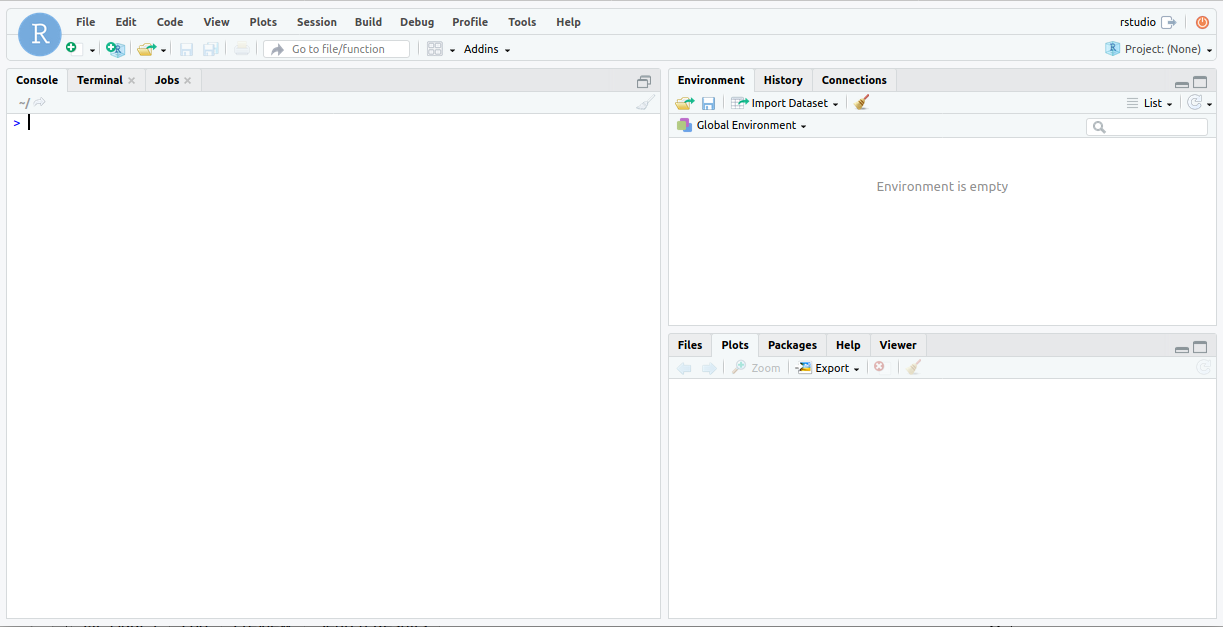
\includegraphics[width=0.8\textwidth]{imagens/RStudio.png}
	\caption{Ambiente do R}
\end{figure}

A primeira (no canto inferior a esquerda) está a janela de comandos (ou \textbf{Console}) na qual podemos digitar um comando separadamente bem como acessar o terminal ou executar um Job.

A segunda (no canto superior a direita) está localizada principalmente a janela de ambiente (\textbf{Environment}) é onde fica exposta todas as variáveis criadas ou bases de dados. A aba \textbf{History} contém um histórico de todos os comandos que foram executados no ambiente, e a aba \textbf{Connections} todas as conexões estabelecidas com diversas bases de dados.

E a terceira (no canto inferior a direita) nos permite acesso principalmente as telas de auxílio (abas \textbf{Help} e \textbf{Viewer}), aos pacotes (aba \textbf{Packages}), aos gráficos criados (aba \textbf{Plots}) e aos arquivos do diretório corrente. Observe que qualquer ação executada nessas abas vai parar na janela de comandos. Se por exemplo, na aba de pacotes solicitamos a instalação de um novo pacote ou na aba de arquivos removemos ou renomeamos um arquivo o comando respectivo é mostrado e executado na console.

\begin{theo}[]{}
A partir deste ponto, todos os comandos aqui mostrados, foram digitados na \textit{Console}: digitar o comando e pressionar Enter, salvo qualquer observação contrária. 
\end{theo}

O principal comando de todo iniciante: \\
{\ttfamily help.start()} 

Na aba \textit{Help} será mostrado diversos manuais, referencias e materiais sobre a linguagem.

Limpar a console de saída usar o comando: \\
{\ttfamily cat("$\setminus$014")}

Podemos também usar no menu: Edit $\triangleright$ Clear Console. É recomendável explorar as opções disponíveis neste menu e se familiarizar com suas opções.

\section{Comandos para Pacotes}
Os pacotes complementam as funções da linguagem e agregam mais poder ao R. 

Instalar um pacote: \\
{\ttfamily install.packages("nome")}

Podemos também utilizar a opção \textit{dependencies} para adicionar automaticamente todas as suas dependências: \\
{\ttfamily install.packages("nome", dependencies=TRUE)}

Por exemplo, um pacote muito comum a ser instalado é o \textbf{dbplyr} (usaremos este como referência para os próximos comandos), para instalar: \\
{\ttfamily install.packages("dbplyr", dependencies=TRUE)}

Obter uma ajuda sobre o pacote: \\
{\ttfamily library(help = "dbplyr")}

Usar o pacote instalado: \\
{\ttfamily library("dbplyr")}

\subsection{Chaining do pacote DPLYR}
R tem suas particularidades como linguagem, uma delas é \textit{chaining} (algo como encadeamento) contido no pacote DPLYR, funciona como uma agregação sequencial de métodos em outras linguagens. Observemos o seguinte exemplo:
\begin{lstlisting}
x1 <- 1:5; x2 <- 2:6
sqrt(sum((x1-x2)^2))
\end{lstlisting}

\begin{theo}[]{}
	Para funcionar esta funcionalidade, devemos habilitar o pacote ``dplyr'': \\
	{\ttfamily library("dplyr")}
\end{theo}

Com \textit{chaining}, reescrevemos a última linha da seguinte forma:
\begin{lstlisting}
x1 <- 1:5; x2 <- 2:6
(x1-x2)^2 %>% sum() %>% sqrt()
\end{lstlisting}

O resultado da primeira expressão é passado para a segunda, e por sua vez para a terceira. O resultado é exatamente o mesmo, mas temos a vantagem de entendermos melhor como procede as ações - sendo este um padrão seguido pela maioria dos usuários.

\section{Básico da Linguagem}
Nessa seção entenderemos como o R funciona, aprender algumas funções e diversos exemplos práticos.

\subsection{Tipos de Dados}
R trabalha com 5 tipos de dados (em R o comando de atribuição é {\ttfamily <-}):
\begin{itemize}
  \item \textbf{Numérico - numeric}: São números com a forma decimal: {\ttfamily a <- 1.6} Obs. Não confunda, mesmo que a variável recebesse o valor 1, continuaria sendo numérica, para verificar o tipo de dado, executar o comando: {\ttfamily class(a)}, ou perguntar se determinada variável é de determinado tipo: {\ttfamily is.numeric(a)} 
  \item \textbf{Inteiro - integer}: São números sem a parte fracionária: {\ttfamily b <- 1L} Obs. Verifique na janela \textit{Environment} que b está com o valor 1L, outra forma de definir uma inteira é por conversão, i.e {\ttfamily b <- as.integer(a)} e teremos o mesmo resultado 
  \item \textbf{Caractere - character}: São letras ou números: {\ttfamily c <- '12ABC'} Obs. Não é possível realizar operações aritméticas com este tipo de variável e não existe a distinção entre aspas duplas ou simples, qualquer uma pode ser utilizada
  \item \textbf{Fator - factor}: é um tipo especial de vetor que nos permite plotar os dados: {\ttfamily d <- factor(c("Masculino", "Feminino", "Masculino"))} Obs. Neste fator temos 2 ocorrências (ou níveis), isso pode ser verificado com os seguintes comandos: {\ttfamily levels(d)} ou {\ttfamily nlevels(d)} sendo que o primeiro mostra as ocorrências e o segundo a quantidade 
  \item \textbf{Lógica - logical}: Podem ser de 2 tipos TRUE ou FALSE: {\ttfamily e <- TRUE} Obs. Lembre-se que a linguagem é \textit{case-sensitive}, ou seja, existe uma diferença entre as letras maiúsculas de minúsculas
\end{itemize}

Na aba \textbf{Environment} é o lugar que as variáveis são armazenadas.

Ver uma lista das variáveis disponíveis: \\
{\ttfamily ls()}

Eliminar uma variável: \\
{\ttfamily rm(nomeVariavel)}

Apagar completamente a \textit{Workspace}: \\
{\ttfamily rm(list = ls())}

Existem também outros tipos usados em R que são chamados de \textit{Atomic Types} (tipos atômicos), são eles:
\begin{itemize}[noitemsep]
  \item \textbf{double}: São números com alta precisão
  \item \textbf{complex}: São números complexos em notação científica
  \item \textbf{raw}: Armazena os bytes correspondente ao valor da variável
\end{itemize}

Por coerção podemos criar facilmente esses tipos, observe o código a seguir:
\begin{lstlisting}
a <- 25.456        # cria 'a' como numeric
b <- as.double(a)  # cria 'b' como double
c <- as.complex(a) # cria 'c' como complex
d <- as.raw(a)     # cria 'd' como raw
\end{lstlisting}

\subsection{Expressões Matemáticas}
R aceita as quatro operações básicas com a utilização dos operadores comuns. E alguns operadores especiais:
\begin{itemize}
  \item \textbf{\%/\%}: Divisão de dois números com o resultado inteiro
  \item \textbf{\%\%}: Resto da divisão de dois números
  \item \textbf{\^}: Exponenciação
\end{itemize}

Bem como algumas funções matemáticas:
\begin{itemize}
  \item \textbf{abs(x)}: Valor absoluto de x
  \item \textbf{log(x, base = y)}: Logaritmo de x na base y, por conveniência ainda existem as funções log2 e log10
  \item \textbf{exp(x)}: Exponencial de x, o contrário do logaritmo
  \item \textbf{sqrt(x)}: Raiz quadrada de x
  \item \textbf{factorial(x)}: Fatorial de x
  \item \textbf{choose(x,y)}: Número de possíveis combinações entre x e y
  \item \textbf{signif(x, digits = y)}: Mostra o elemento x com o máximo de digitos informados em y
\end{itemize}

Por exemplo para calcular o logaritmo de 1 a 3 na base 10:
\begin{lstlisting}
x <- log(1:3)
exp(x)
\end{lstlisting}

\subsection{Lidar com Strings}
Não existe qualquer problema entre usar aspas duplas ou simples, porém para o iniciante a linguagem pode parecer esquisita ao não permitir uma simples concatenação envolvendo duas Strings: \\
{\ttfamily nomeCompleto = 'Fernando' + 'Anselmo'}

Resolvido ao utilizar o comando \textbf{paste}: \\
{\ttfamily nomeCompleto = paste('Fernando', 'Anselmo')}

Observamos que um espaço entre as strings é inserido automaticamente: \\
{\ttfamily print(nomeCompleto)}

Porém em alguns casos não desejamos que isso aconteça, resolvemos com a opção \textbf{sep}: \\
{\ttfamily nomeCompleto = paste("Fernando", "Anselmo", sep = '')}

Contar quantos caracteres uma determinada String possui: \\
{\ttfamily nchar(nomeCompleto)}

Obter parte de uma String (o primeiro carácter está na posição 0): \\
{\ttfamily substring(nomeCompleto, 4, 8)}

\subsection{Vetores}
Um vetor (vector) em R é uma combinação de elementos de mesmo tipo.

Criar um vetor: \\
{\ttfamily c("coração", "espada", "copas", "paus")}

Guardar o vetor em uma variável: \\
{\ttfamily tc <- c("coração", "espada", "copas", "paus")}

Trazer o valor do segundo elemento, ou seja ``espada''. Utilizamos seu índice entre colchetes. O primeiro elemento possui o índice 1 e assim sucessivamente: \\
{\ttfamily tc[2]}

Obter vários elementos (no caso três) usamos o operador de intervalo: \\
{\ttfamily tc[2:4]}

Juntar valores caracteres: \\
{\ttfamily paste("Tipo de carta:", tc[1:4])}

Obter o tamanho de um vetor: \\
{\ttfamily length(tc)}

Outra forma de se criar um vetor seria através de um intervalo, por exemplo, para definir um vetor cartas com 13 elementos de 1 a 13: \\
{\ttfamily vc <- c(1:13)}

Outro detalhe interessante com vetores é que podemos proceder operações em 
conjunto, veja esses exemplos:
\begin{lstlisting}
vc <- vc + 2          # Somar um valor a todos os elementos
vc <- vc + 2:4        # Somar uma sequencia repetidamente nos elementos
vc <- vc * 2          # Multiplicar um valor por todos os elementos
vc <- vc / 2          # Dividir um valor por todos os elementos
vc <- vc[-c(5,6)]     # Remover os elementos em determinadas posicoes
vc[1] <- 5            # Trocar o valor do primeiro elemento
vc[1:4] <- 5          # Trocar o valor em determinadas posicoes
vc[length(vc)+1] <- 8 # Adicionar um valor ao final do vetor 
vc <- sort(vc)        # Reordenar o vetor
vc[which(vc > 7)]     # Mostrar valores por uma condicao determinada
rm(vc)                # remover o vetor
\end{lstlisting}

Nomear cada um dos elementos de um vetor, por exemplo, para definir o período percorrido em corridas realizadas a cada dia da semana:
\begin{lstlisting}
dias <- c("Seg", "Ter", "Qua", "Qui", "Sex", "Sab", "Dom")
kms <- c(1.5, 2.3, 2.3, 3.2, 2.2, 1.8, 1.2)
names(kms) <- dias
kms # mostra o resultado do vetor com seus labels definidos

# Outra forma mais simples, com o mesmo resultado, seria:
kms <- c(Seg = 1.5, Ter = 2.3, Qua = 2.3, Qui = 3.2, 
         Sex = 2.2, Sab = 1.8, Dom = 1.2)
         
# Trazer o valor de um elemento:
kms[2]      # valor do segundo elemento
kms["Ter"]  # ou pelo seu nome
\end{lstlisting}

Na segunda forma as aspas são opcionais. Outras funções também utilizadas com vetores:
\begin{lstlisting}
head(NomeVetor)   # Mostra os dados iniciais do vetor
tail(NomeVetor)   # Mostra os dados finais do vetor
\end{lstlisting}

\subsection{Análise de dados com Vetores}
Obtermos informações sobre o vetor: \\
{\ttfamily str(kms)}

Realizar uma análise de seus dados é essencial conhecer algumas funções básicas de estatística e aritmética:
\begin{lstlisting}
sum(kms)           # Soma dos Kms percorridos na semana
sort(kms)          # Ordenar os Kms percorridos na semana
mean(kms)          # Media dos Kms percorridos na semana
max(kms)           # Maior Km percorrido
min(kms)           # Menor Km percorrido
median(kms)        # Media ponderada dos Kms percorridos na semana
sd(kms)            # Desvio padrao
log(kms)           # Logaritmo de cada Km
dnorm(kms)         # Probabilidade da densidade da distribuicao normal
pnorm(kms)         # Integral para -infinito da distribuicao normal
rnorm(kms)         # Vetor da distribuicao de numeros randomicos
dlnorm(kms)        # Logaritmo da distribuicao normal de cada Km
sqrt(kms)          # Raiz Quadrada de cada Km
quantile(kms)      # Quantil, dividos em pontos de 25%
quantile(kms, .25) # Primeiro Quartil ou quartil inferior
quantile(kms, .50) # Segundo Quartil (ou a mediana)
quantile(kms, .75) # Terceiro Quartil ou quartil superior
quantile(kms, 1)   # Quarto Quartil (ou a maxima)
summary(kms)       # Resumo dos dados do vetor
\end{lstlisting}

Para explicar melhor, vamos ver o real poder do R e traduzir algumas dessas informações em formato gráfico:
\begin{lstlisting}
boxplot(kms)        # Cria um grafico do resumo dos dados (summary)

# So isso... Entendamos o que significa cada separacao...
abline(h = min(kms), col = "Blue")
abline(h = max(kms), col = "Yellow")
abline(h = median(kms), col = "Green")
abline(h = quantile(kms, c(0.25, 0.75)), col = "Red")
\end{lstlisting}

E o resultado será:
\begin{figure}[H]
	\centering
	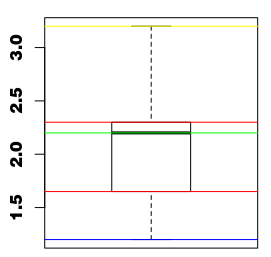
\includegraphics[width=0.3\textwidth]{imagens/grafico01.png}
	\caption{Resultado da Expressão}
\end{figure}

A caixa no meio do gráfico, formada pelos 1º e 3º quartis, em estatística é conhecida por ``Intervalo interquartil''. Dados fora dessa caixa podem ser considerados discrepantes, por exemplo o máximo km percorrido foi 3,2 porém ocorreu somente uma vez, assim como o menor km percorrido foi 1,2. Se repararmos os dados, os valores medianos estão entre 1,65 e 2,30 que correspondem exatamente a esse intervalo.

A função ``Quantil'' (quantile()) nos permite analisar outros dados interessantes. O primeiro seria dividir os valores em 10 partes (com intervalos de 10\%), isso é chamado de ``decil'' (que é qualquer valor da divisão de uma 
variável em 10 partes iguais): \\
{\ttfamily quantile(kms, prob = seq(0, 1, length = 11), type = 5)}

E com esse conhecimento, podemos localizar qualquer ``percentil'' que desejarmos, um percentil é uma medida estatística que divide uma amostra em 100 partes, cada uma com uma percentagem de dados é aproximadamente igual. Por exemplo, para acharmos o 32º, 57º e 98º percentil na nossa corrida semanal, podemos usar: \\
{\ttfamily quantile(kms, prob = c(.32, .57, .98))}

Outro gráfico muito simples de ser realizado é a plotagem: \\
{\ttfamily plot(kms)}

E o resultado será este:
\begin{figure}[H]
	\centering
	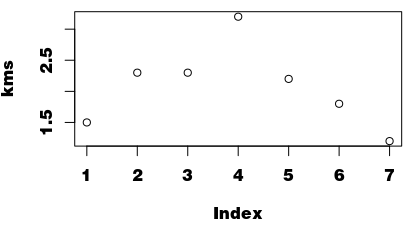
\includegraphics[width=0.4\textwidth]{imagens/grafico03.png}
	\caption{Resultado da Expressão}
\end{figure}

Porém um histograma é bem mais interessante para a Análise de Dados: \\
{\ttfamily hist(kms)}

E o resultado será este:
\begin{figure}[H]
	\centering
	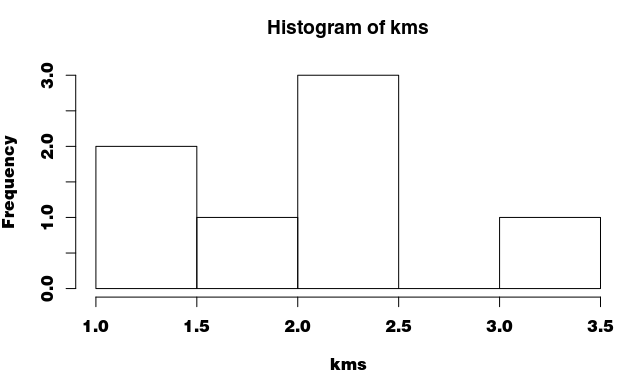
\includegraphics[width=0.4\textwidth]{imagens/grafico02.png}
	\caption{Resultado da Expressão}
\end{figure}

Um histograma mostra os dados de forma agrupada por intervalos regulares, neste caso observamos que entre 1 km e 1,5 km a frequência foi de 2 vezes (ocorreu no Domingo e na Segunda), entre 1,5 km e 2 km a frequência foi 1 vez (ocorreu no Sábado) e assim se procede sua leitura.

Por fim podemos utilizar o ``Normal-Quantile Plots'' para traçar um gráfico com a distribuição padrão normal dos nossos dados e verificar qual nossa média real de quilômetros percorridos na corrida:
{\ttfamily qqnorm(kms)}

E o resultado será este:
\begin{figure}[H]
	\centering
	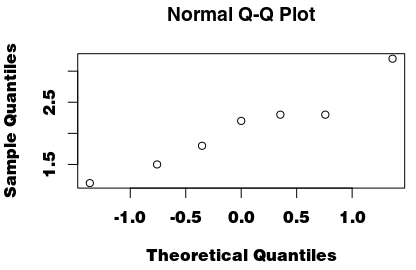
\includegraphics[width=0.4\textwidth]{imagens/grafico04.png}
	\caption{Resultado da Expressão}
\end{figure}

Observamos que no padrão linear deste gráfico que a maior concentração de pontos se concentra entre 1,5 Km e 2,5 Km.

\subsection{Limpar Vetores}
O maior trabalho do ``Analista de Dados'' é o de organizar as amostras para que os dados fiquem coerentes. O primeiro caso é no qual os vetores podem conter (devido a diversas operações realizadas) valores ``não é valor'', em R são reconhecidos por \textbf{NA}, veja a seguinte simulação:
\begin{lstlisting}
a <- c(1:10) # criar um vetor A com 10 elementos
a[2] <- NA   # atribuir para o elemento 2 o valor NA
a[6] <- NA   # atribuir para o elemento 6 o valor NA
\end{lstlisting}

Obviamente isto é apenas um exemplo, sendo que o vetor ``a'' contém os seguintes valores: \\
{\ttfamily 1 NA  3  4  5 NA  7  8  9 10}

É impossível aplicar as funções vistas neste vetor. Para limpá-lo podemos utilizar o seguinte comando: \\
{\ttfamily a <- na.omit(a)}

E todos os valores NA serão retirados. Outra forma que fará o mesmo efeito é: \\
{\ttfamily a <- a[!is.na(a)]}

Verificar os dados: \\
{\ttfamily any(is.na(a))}

E será retornado FALSE, indicando que a nossa amostra está coerente. 

A segunda forma é bem interessante, imaginemos agora o seguinte vetor: \\
{\ttfamily numFilhos <- c(5, 2, -3, 1, 0, -4)}

Remover todos os valores negativos deste vetor, que apresentam erros na amostragem: \\
{\ttfamily numFilhos <- numFilhos[numFilhos > 0]}

Operações básicas de lógica em R:
\begin{lstlisting}
any(logical)   # Retorna TRUE ou FALSE dependendo da analise logica
is.[tipo](var) # Se a variavel eh de determinado tipo
>              # Maior que
<              # Menor que
>=             # Maior ou igual a
<=             # Menor ou igual a
==             # Igual a
!=             # Nao igual a
\end{lstlisting}

\subsection{Números Aleatórios}
Gerar uma sequencia de 10 números aleatórios: \\
{\ttfamily runif(10)}

Limitar os valores mínimo e máximo: \\
{\ttfamily runif(10, min = 5, max = 50)}

Definir a quantidade de casas decimais: \\
{\ttfamily options(digits = 2)}

Gerar um vetor de 10 letras aleatórias: \\
{\ttfamily letters[round(runif(10, min = 1, max = 27))]}

E em maiúsculas: \\
{\ttfamily LETTERS[round(runif(10, min = 1, max = 27))]}

Resumo das Funções:
\begin{lstlisting}
runif(n, max, min) # Gera numeros aleatorios
options()          # Define diversas saidas
round(n)           # Arredonda para o mais proximo inteiro
letters ou LETTERS # Vetor com as letras do alfabeto minusculas e maiusculas
\end{lstlisting}

\section{Pacote DPLYR}
Na subseção de Chaining foi mostrado um dos comandos do pacote DPLYR, vamos nos aprofundar mais nele para entender melhor seu funcionamento. Basicamente serve como substituição de muitas funções de acesso a \textit{DataSet}. 

Instalar o \textit{DataSet} \textbf{hflights}: \\
{\ttfamily install.packages(c("hflights", "Lahman"))}

Usar ambos pacotes: \\
{\ttfamily library(dplyr)} \\
{\ttfamily library(hflights)}

Utilizar o \textit{DataSet} de Voos: \\
{\ttfamily voos <- tibble::as\_tibble(hflights)}

Visualizar a estrutura de um objeto, normalmente usaríamos o comando \textit{str(voos)}, com o pacote \textbf{dplyr} ativo usaremos: \\
{\ttfamily glimpse(voos)}

\subsection{Seleções}
Selecionar determinadas colunas: \\
{\ttfamily select(voos, DepTime, ArrTime, FlightNum)}

Selecionar determinadas colunas, por um vetor:
\begin{lstlisting}
cols <- c("Year", "Month", "DayofMonth")
voos %>% 
  select(one_of(cols))
\end{lstlisting}

Selecionar determinadas colunas que contenham tal expressão: \\
{\ttfamily select(voos, Year:DayofMonth, contains("Taxi"), contains("Delay"))} 

Seleção distinta, sem repetições:
\begin{lstlisting}
voos %>% 
  select(Year, Month) %>%
  distinct()
\end{lstlisting}

Obter, aleatoriamente, uma amostra de X linhas:
\begin{lstlisting}
voos %>%
  sample_n(5)
\end{lstlisting}

Obter, aleatoriamente, uma amostra de uma fração linhas:
\begin{lstlisting}
voos %>%
  sample_frac(0.08, replace = TRUE)
\end{lstlisting}

Obter somente os campos numéricos:
\begin{lstlisting}
voos %>% 
  summarise_if(is.numeric, mean, na.rm = TRUE)
\end{lstlisting}

Três exemplos de todas as colunas, menos algumas:
\begin{lstlisting}
voos %>% select(-Month, -DayofMonth)        # determinadas
voos %>% select(-(UniqueCarrier:Cancelled)) # intervalo
voos %>% select(-contains("time"))          # determinado termo 
\end{lstlisting}

Renomear colunas:
\begin{lstlisting}
# Somente as renomeadas aparecem
voos %>% 
  select(Origem = Origin, Destino = Dest, Distancia = Distance)
# Todas as colunas aparecem, inclusive as renomeadas
voos %>% 
  rename(Origem = Origin, Destino = Dest, Distancia = Distance)
\end{lstlisting}

\subsection{Filtragens}
Obter todos os Voos de um determinado Mês E Ano: \\
{\ttfamily filter(voos, Month == 1 \& DayofMonth==1)}

Obter todos os Voos de determinados Transportadores: \\
{\ttfamily filter(voos, UniqueCarrier == 'AA' | UniqueCarrier == 'UA')}

Também podemos utilizar: \\
{\ttfamily filter(voos, UniqueCarrier \%in\% c('AA','UA'))}

Mesclar SELEÇÃO e FILTRO:
\begin{lstlisting}
voos %>%
  select(UniqueCarrier, DepDelay) %>%
  filter(DepDelay > 60)
\end{lstlisting}

Mesclar SELEÇÃO e FILTRO:
\begin{lstlisting}
voos %>% 
  filter(DepTime >= 600, DepTime <= 605)
voos %>% 
  filter(between(DepTime, 600, 605))
voos %>% 
  filter(!is.na(DepTime))
\end{lstlisting}

Fatiar:
\begin{lstlisting}
voos %>% 
  slice(1000:1005)
voos %>% 
  filter(!is.na(DepTime)) %>% slice(1000:1005)
\end{lstlisting}

\subsection{Agrupamentos}
Por destino, calcular a média de voos:
\begin{lstlisting}
voos %>%
  group_by(Dest) %>%
  summarise_all(mean, na.rm = TRUE)
\end{lstlisting}

Por destino, calcular a média de voos atrasados:
\begin{lstlisting}
voos %>%
  group_by(Dest) %>%
  summarise_at(vars(c("ArrDelay")), mean, na.rm = TRUE)
\end{lstlisting}

Por transporte, contar a porcentagem de voos cancelados ou desviados:
\begin{lstlisting}
voos %>%
  group_by(UniqueCarrier) %>%
  summarise_at(vars(c("Cancelled","Diverted")), mean, na.rm = TRUE)
\end{lstlisting}

Por transporte, contar o mínimo ou máximo, de chegadas ou partidas, atrasadas:
\begin{lstlisting}
voos %>%
  group_by(UniqueCarrier) %>%
  summarise_at(vars(matches("Delay")), funs(min, max), na.rm = TRUE)
\end{lstlisting}

Por dia, contar o total de voos (ordenados descendentemente):
\begin{lstlisting}
voos %>%
  group_by(Month, DayofMonth) %>%
  tally(sort = TRUE)
\end{lstlisting}

Por destino, contar o total de voos e o número de aeronaves (sem repetição):
\begin{lstlisting}
voos %>%
  group_by(Dest) %>%
  summarise(FlightCount = n(), PlaneCount = n_distinct(TailNum))
\end{lstlisting}

Três de cada grupo (Ordenado pelo Horário da Partida)
\begin{lstlisting}
voos %>% 
  group_by(Month, DayofMonth) %>% 
  top_n(3, DepTime) 
\end{lstlisting}

Três de cada grupo (Ordenado pelo Horário da Partida descendentemente)
\begin{lstlisting}
voos %>% 
  group_by(Month, DayofMonth) %>% 
  top_n(3, DepTime) %>% 
  arrange(Month, DayofMonth, desc(DepTime))
\end{lstlisting}

Por destino, contar o total de cancelados e não cancelados:
\begin{lstlisting}
voos %>%
  group_by(Dest) %>%
  select(Cancelled) %>%
  table() %>%
  head()
\end{lstlisting}

Fatiar:
\begin{lstlisting}
# 3 primeiras de cada Grupo
voos %>% 
  group_by(Month, DayofMonth) %>% 
  slice(1:3)
# 3 de cada grupo (aleatoriamente)
voos %>% 
  group_by(Month, DayofMonth) %>% 
  sample_n(3)
\end{lstlisting}

\subsection{Agregações}
Para cada transporte, calcular a cada dois dias, a partida mais atrasada:
\begin{lstlisting}
voos %>%
  group_by(UniqueCarrier) %>%
  select(Month, DayofMonth, DepDelay) %>%
  top_n(2) %>%
  arrange(UniqueCarrier, desc(DepDelay))
\end{lstlisting}

Para cada mês, o total de voos e as mudanças do mês anterior:
\begin{lstlisting}
voos %>%
  group_by(Month) %>%
  tally() %>%
  mutate(change = n - lag(n))
\end{lstlisting}

\subsection{Mutações e Transmutações}
Mutações são novos campos que não existem no \textit{DataSet} original. Podemos utilizá-los sem modificar o \textit{DataSet}, da seguinte forma:
\begin{lstlisting}
voos %>%
  select(Distance, AirTime) %>%
  mutate(Velocidade = Distance / AirTime*60)
\end{lstlisting}

Ou modificar o DataSet, da seguinte forma:
\begin{lstlisting}
voos <- voos %>% 
  mutate(Velocidade = Distance / AirTime*60)
select(voos, Distance, Velocidade)
\end{lstlisting}

Transmutação apenas a coluna criada aparecerá:
\begin{lstlisting}
voos %>% 
  transmute(Velocidade = Distance / AirTime * 60)
\end{lstlisting}

\section{Lidar com Arquivos Externos}
Obviamente boa parte do trabalho de um Cientista de Dados é ler arquivos externos (principalmente do tipo CSV) para realizar suas analises, como proceder essa leitura já que estamos em um contêiner Docker? Lembramos que quando foi criado o contêiner este foi associado a uma pasta (através da diretiva volume: {\ttfamily -v \$HOME/rstudio:/home/rstudio}), assim basta apenas colocar o arquivo nessa pasta é proceder sua leitura normalmente.

Ler o arquivo titanic.csv: \\
{\ttfamily titanic <- read.csv(file = 'titanic.csv')}

Verificar os dados: \\
{\ttfamily head(titanic)}

Outras vezes podemos necessitar em gerar um arquivo PDF de um gráfico, por exemplo:
\begin{lstlisting}
a <- 2
b <- -3
sigSq <- 0.5
x <- runif(40)
y <- a + b * x + rnorm(40, sd = sqrt(sigSq))
(avgX <- mean(x))
write(avgX, "avgX.txt")
plot(x, y)
abline(a, b, col = "red")
dev.print(pdf, "meugrafico.pdf")
\end{lstlisting}

\begin{theo}[]{}
Nos exemplos abaixo trocar o termo [URL] para \\ \url{https://raw.githubusercontent.com/fernandoans/machinelearning/master/bases}
\end{theo}

Observamos que o arquivo gerado foi criado no seu sistema (fora do contêiner). Também podemos trazer dados da Web sem o menor problema, por exemplo: \\
{\ttfamily x <- scan("[URL]/gameML.txt", what = list(nome = "", familia = "", idade = 0, salario = 0.0))}

O maior problema nessa maneira é que os dados devem estar corretamente organizados (sem a falta de informações), note que a opção \textbf{what} mostra como estão estruturados. Se existe um cabeçalho podemos utilizar a opção \textbf{header = TRUE}.

Podemos utilizar o seguinte modo para trazer um arquivo texto, onde cada linha será um registro:
{\ttfamily y <- scan("[URL]//cbcNewsOct2.srt", what = character(), sep = '$\setminus$n')}

Trazer um arquivo CSV da Web:
{\ttfamily game.csv <- read.csv("[URL]/gameML.csv", header = TRUE, sep = ";")}

Listar o arquivo:
{\ttfamily print(game.csv)}

Gravar um arquivo:
{\ttfamily write.table(game.csv, file.path(getwd(), "saida.txt"), col.names = FALSE, row.names = FALSE, quote = TRUE)}

Tiramos o cabeçalho e os nomes (índices) das colunas e adicionamos aspas para os caracteres assim podemos facilmente ler:
{\ttfamily x <- scan("saida.txt", what = list(nome = "", idade = 0, salario = 0.0))}

\section{Conclusão}
O objetivo desta apostila foi o de mostrar como iniciar seus estudos na Linguagem R é não de ensinar estatística. Foi planejada para ser usada durante disciplinas com o uso da linguagem R (principalmente para pessoas que nunca usaram o R), mas isso não impede que seja utilizada em diversas fases de seus estudos.

A maioria dos pacotes tem por objetivo análises estatísticas, porém praticamente qualquer aplicativo que exista pode ser portado para R. Apesar de R ser usada, primariamente, para análises estatísticas, é uma linguagem de programação completa, capaz de realizar qualquer tarefa que outras linguagens realizam. A evolução e amadurecimento do R, tem levado grandes empresas como Oracle e Microsoft, a investirem seus bilionários recursos em pesquisa e desenvolvimento para aprimorar suas soluções analíticas utilizando o R como base. A linguagem R vem se tornando ainda o principal ``idioma'' de Cientistas e Analistas de Dados e está liderando a revolução proporcionada por \textit{Big Data Analytics}.

R é uma das linguagens de computador que mais cresce no mundo. Parte devido ao crescente comunidade de usuários que contribui com pacotes, que são conjuntos de pequenos programas que expandem suas funcionalidades. No Brasil, contamos com espelhos na USP, UFPR e fundação Oswaldo Cruz. ``R é uma demonstração real do poder da colaboração, e não creio que fosse possível criar algo parecido de qualquer outra maneira'', disse Ihaka. ``Se tivéssemos escolhido lançar o software como produto comercial, teríamos vendido cinco cópias''. 

Sou um entusiasta do mundo \textbf{Open Source} e novas tecnologias. Qual a diferença entre Livre e Open Source? \underline{Livre} significa que esta apostila é gratuita e pode ser compartilhada a vontade. \underline{Open Source} além de livre todos os arquivos que permitem a geração desta (chamados de arquivos fontes) devem ser disponibilizados para que qualquer pessoa possa modificar ao seu prazer, gerar novas, complementar ou fazer o que quiser. Os fontes da apostila (que foi produzida com o LaTex) está disponibilizado no GitHub \cite{github}, assim baixar, alterar e usar. Veja ainda outros artigos que publico sobre tecnologia através do meu Blog Oficial \cite{fernandoanselmo}.

%-----------------------------------------------------------------------------
% REFERÊNCIAS
%-----------------------------------------------------------------------------
\begin{thebibliography}{5}
  \bibitem{cranoficial} 
  Página do CRAN \\
  \url{http://cran.r-project.org/}
  
  \bibitem{rstudiooficial} 
  Página do RStudio \\
  \url{https://www.rstudio.com/}
  
  \bibitem{fernandoanselmo} 
  Fernando Anselmo - Blog Oficial de Tecnologia \\
  \url{http://www.fernandoanselmo.blogspot.com.br/}

  \bibitem{publicacao} 
  Encontre essa e outras publicações em \\
  \url{https://cetrex.academia.edu/FernandoAnselmo}

  \bibitem{github} 
  Repositório para os fontes da apostila \\
  \url{https://github.com/fernandoans/publicacoes}
\end{thebibliography}
  
\end{document}
